\documentclass[a4paper,11pt,titlepage]{jsarticle}
\usepackage{amsmath,amssymb}
\usepackage{bm}
\usepackage[dvipdfmx]{graphicx}
\usepackage{here}

%テキストの表示領域の調節
\setlength{\textwidth}{\paperwidth}
\addtolength{\textwidth}{-40truemm}
\setlength{\textheight}{\paperheight}
\addtolength{\textheight}{-45truemm}

%余白の調節
\setlength{\topmargin}{-10.4truemm}
\setlength{\evensidemargin}{-5.4truemm}
\setlength{\oddsidemargin}{-5.4truemm}
\setlength{\headheight}{17pt}
\setlength{\headsep}{10mm}
\addtolength{\headsep}{-17pt}
\setlength{\footskip}{5mm}

\title{4.ロボットの制御}
\author{1610004 青木 良太}
\date{2018年6月21日} % 省略可
\begin{document}
\maketitle

\section{実験の目的}
ロボットを用いて各種制御実験を行い,ロボットの各種制御法,運動学,動力学,冗長性について理解する.
\section{実験課題}
2リンクのロボットアームを対象として,制御方法の種類,目標値の種類,ゲインの大小,モデル誤差の有無を変更し,シミュレーションを行った.
制御方法はPD制御,重力補償つきPD制御,フィードバック線形化の3つから選択した.目標値は時不変目標値(PTP制御)と時変目標値(軌道追従制御)の2つから選択した.
ゲインの設定は大,中,小の3つから選択でき,モデル誤差は有,無の2つから選択した.

\subsection{課題1}
目標値が時不変,モデル誤差無しの場合について,各種制御を実行した.
その結果を以下に示す.

\begin{figure}[H]
  \begin{center}
    \includegraphics[width = 10cm]{画像/eps_関節_PD_時不変_小_モデル誤差なし_時間応答.eps}
    \caption{制御法:PD制御,ゲイン:小}
    \label{PD/ゲイン小}
  \end{center}
\end{figure}

\begin{figure}[H]
  \begin{center}
    \includegraphics[width = 10cm]{画像/eps_関節_PD_時不変_中_モデル誤差なし_時間応答.eps}
    \caption{制御法:PD制御,ゲイン:中}
    \label{PD/ゲイン中}
  \end{center}

\end{figure}
\begin{figure}[H]
  \begin{center}
    \includegraphics[width = 10cm]{画像/eps_関節_PD_時不変_大_モデル誤差なし_時間応答.eps}
    \caption{制御法:PD制御,ゲイン:大}
    \label{PD/ゲイン大}
  \end{center}
\end{figure}

\begin{figure}[H]
  \begin{center}
    \includegraphics[width = 10cm]{画像/eps_関節_重力補償つきPD_時不変_小_モデル誤差なし_時間応答.eps}
    \caption{制御法:重力補償付きPD制御,ゲイン:小}
    \label{PDG/ゲイン小}
  \end{center}
\end{figure}

\begin{figure}[H]
  \begin{center}
    \includegraphics[width = 10cm]{画像/eps_関節_重力補償つきPD_時不変_中_モデル誤差なし_時間応答.eps}
    \caption{制御法:重力補償付きPD制御,ゲイン:中}
    \label{PDG/ゲイン中}
  \end{center}
\end{figure}

\begin{figure}[H]
  \begin{center}
    \includegraphics[width = 10cm]{画像/eps_関節_重力補償つきPD_時不変_大_モデル誤差なし_時間応答.eps}
    \caption{制御法:重力補償付きPD制御,ゲイン:大}
    \label{PDG/ゲイン大}
  \end{center}
\end{figure}

\begin{figure}[H]
  \begin{center}
    \includegraphics[width = 9cm]{画像/eps_関節_FB線形化_時不変_小_モデル誤差なし_時間応答.eps}
    \caption{制御法:フィードバック線形化制御,ゲイン:小}
    \label{FB/ゲイン小}
  \end{center}
\end{figure}

\begin{figure}[H]
  \begin{center}
    \includegraphics[width = 10cm]{画像/eps_関節_FB線形化_時不変_中_モデル誤差なし_時間応答.eps}
    \caption{制御法:フィードバック線形化制御,ゲイン:中}
    \label{FB/ゲイン中}
  \end{center}
\end{figure}

\begin{figure}[H]
  \begin{center}
    \includegraphics[width = 10cm]{画像/eps_関節_FB線形化_時不変_大_モデル誤差なし_時間応答.eps}
    \caption{制御法:フィードバック線形化制御,ゲイン:大}
    \label{FB/ゲイン大}
  \end{center}
\end{figure}

各制御法において,ゲイン小から大へのグラフの変化を見ると,ゲインが大きくなるにつれ目標値への到達時間が短くなり,
オーバーシュート量も小さくなっていっている.同時に,モータの出力($\tau_1$,$\tau_2$)の最大値も比例して増加していることがわかる.
ゲイン中の場合でそれぞれの制御法を行った場合(図\ref{PD/ゲイン中},図\ref{PDG/ゲイン中},図\ref{FB/ゲイン中})を比べると,
目標値への到達はFB線形化, 重力補償つきPD制御, PD制御の順に速く, モータの出力の最大値は, FB制御, 重力補償つきPD制御, PD制御の順に大きい.
この傾向はゲイン小,大の場合にも同様に見られるが,ゲイン大の場合では,目標到達時間がPD制御においてはオーバーシュートが残っているものの,全ての制御において有意な差は見られなかった.
\par
課題1で得られた結果から良好なものを選定する.良好な結果の定義として,オーバーシュート量が小さいこと,目標到達時間が速い,加えるモータの仕事が小さいことである.
ロボットアームの機能として, 精度が第一に優先されるため,オーバーシュートが微小なものを選定すると,FB線形化(ゲイン:小中大),重力補償つきPD制御(ゲイン:小中大)となる.
次点で,過度なモータ出力(800〜1000 N・m)は実機での動作が困難であることを考慮すると, FB線形化(ゲイン:小中),重力補償つきPD制御(ゲイン:小中大)が残る.
ここで,目標到達時間を$t$,モータの出力の最大値を$\tau$として,二つの積$\alpha$を定義し結果を評価する.
$\alpha$が小さいほど少ない出力である上に目標到達時間が速く,良好な結果であると考えられる.
\begin{align}
  \alpha = t\times\tau
\end{align}
FB線形化(ゲイン:小中),重力補償つきPD制御(ゲイン:小中大)においてそれぞれ目標到達時間とモータの出力効率を以下の表にまとめた.
この時, $\tau$は$\tau1,\tau2$の最大値の平均値をとった.
\begin{table}[H]
	\caption{時不変,モデル誤差無しの場合の結果比較}
	\label{時不変,モデル誤差無しの場合の結果比較}
	\begin{center}
		\begin{tabular}{c|c|c|c|c}\hline
		   & $\tau_1$の最大値 & $\tau_2$の最大値 & 目標到達時間 & $\alpha$ \\ \hline
			重力補償つきPD制御(ゲイン小) & 17.0 & 7.60 & 14.0 & 172.2\\ \hline
			重力補償つきPD制御(ゲイン中) & 27.5 & 17.5 & 3.70 &  83.25\\ \hline
      重力補償つきPD制御(ゲイン大) & 270 & 260 & 1.50 & 397.5 \\ \hline
      FB線形化(ゲイン小) & 35.0 & 8.50 & 3.70 & 80.48 \\ \hline
      FB線形化(ゲイン中) & 80.0 & 20.5 & 1.25 & 62.81 \\ \hline
	   \end{tabular}
\end{center}
\end{table}

表\ref{時不変,モデル誤差無しの場合の結果比較}から,時不変,モデル誤差無しの場合では
FB線形化(ゲイン中), FB線形化(ゲイン小), 重力補償つきPD制御(ゲイン中)の3つが順に良好な結果だと考えられる.

\subsection{課題2}
目標値が時変の場合について,各種制御方法を実行し,結果を観察した.
その結果を以下に示す.

\begin{figure}[H]
  \begin{center}
    \includegraphics[width = 10cm]{画像/eps_関節_PD_時変_小_モデル誤差なし_時間応答.eps}
    \caption{制御法:PD制御,ゲイン:小}
    \label{変/PD/ゲイン小}
  \end{center}
\end{figure}

\begin{figure}[H]
  \begin{center}
    \includegraphics[width = 10cm]{画像/eps_関節_PD_時変_中_モデル誤差なし_時間応答.eps}
    \caption{制御法:PD制御,ゲイン:中}
    \label{変/PD/ゲイン中}
  \end{center}

\end{figure}
\begin{figure}[H]
  \begin{center}
    \includegraphics[width = 10cm]{画像/eps_関節_PD_時変_大_モデル誤差なし_時間応答.eps}
    \caption{制御法:PD制御,ゲイン:大}
    \label{変/PD/ゲイン大}
  \end{center}
\end{figure}

\begin{figure}[H]
  \begin{center}
    \includegraphics[width = 10cm]{画像/eps_関節_重力補償つきPD_時変_小_モデル誤差なし_時間応答.eps}
    \caption{制御法:重力補償付きPD制御,ゲイン:小}
    \label{変/PDG/ゲイン小}
  \end{center}
\end{figure}

\begin{figure}[H]
  \begin{center}
    \includegraphics[width = 10cm]{画像/eps_関節_重力補償つきPD_時変_中_モデル誤差なし_時間応答.eps}
    \caption{制御法:重力補償付きPD制御,ゲイン:中}
    \label{変/PDG/ゲイン中}
  \end{center}
\end{figure}

\begin{figure}[H]
  \begin{center}
    \includegraphics[width = 10cm]{画像/eps_関節_重力補償つきPD_時変_大_モデル誤差なし_時間応答.eps}
    \caption{制御法:重力補償付きPD制御,ゲイン:大}
    \label{変/PDG/ゲイン大}
  \end{center}
\end{figure}

\begin{figure}[H]
  \begin{center}
    \includegraphics[width = 10cm]{画像/eps_関節_FB線形化_時変_小_モデル誤差なし_時間応答.eps}
    \caption{制御法:フィードバック線形化制御,ゲイン:小}
    \label{変/FB/ゲイン小}
  \end{center}
\end{figure}

\begin{figure}[H]
  \begin{center}
    \includegraphics[width = 10cm]{画像/eps_関節_FB線形化_時変_中_モデル誤差なし_時間応答.eps}
    \caption{制御法:フィードバック線形化制御,ゲイン:中}
    \label{変/FB/ゲイン中}
  \end{center}
\end{figure}

\begin{figure}[H]
  \begin{center}
    \includegraphics[width = 10cm]{画像/eps_関節_FB線形化_時変_大_モデル誤差なし_時間応答.eps}
    \caption{制御法:フィードバック線形化制御,ゲイン:大}
    \label{変/FB/ゲイン大}
  \end{center}
\end{figure}

各制御法において,ゲイン小から大へのグラフの変化を見ると,不時変の場合と同様に,ゲインが大きくなるにつれ目標値への到達時間が短くなり,
オーバーシュート量も小さくなっていっている.同時に,モータの出力{$\tau_1$,$\tau_2$)の最大値も比例して増加していることがわかる.
ゲイン中の場合でそれぞれの制御法を行った場合(図\ref{変/PD/ゲイン中},図\ref{変/PDG/ゲイン中},図\ref{変/FB/ゲイン中})を比べると,
目標値への到達はFB線形化, 重力補償つきPD制御, PD制御の順に速く, モータの出力の最大値は, PD制御, FB制御,重力補償つきPD制御の順に大きい.
\par
課題2で得られた結果から良好なものを課題1と同様に選定する. オーバーシュートが微小なものを選定すると,PD制御(ゲイン:大), 重力補償つきPD制御(ゲイン:大), FB線形化(ゲイン:小中大)となる.
過度なモータ出力(800〜1000 N・m)は実機での動作が困難であることを考慮すると, FB線形化(ゲイン:小中)が残る.
これらの結果を目標到達時間とモータの出力の最大値の積で結果を評価していく.

FB線形化(ゲイン:小中)においてそれぞれ目標到達時間とモータの出力効率を以下の表にまとめた.
\begin{table}[H]
	\caption{時変,モデル誤差無しの場合の結果比較}
	\label{時変,モデル誤差無しの場合の結果比較}
	\begin{center}
		\begin{tabular}{c|c|c|c|c}\hline
		   & $\tau_1$の最大値 & $\tau_2$の最大値 & 目標到達時間 & $\alpha$ \\ \hline
      FB線形化(ゲイン小) & 27.0 & 17.5 & 3.00 & 66.75 \\ \hline
      FB線形化(ゲイン中) & 34.0 & 50.0 & 1.25 & 52.50 \\ \hline
	   \end{tabular}
\end{center}
\end{table}

表\ref{時変,モデル誤差無しの場合の結果比較}から,時変,モデル誤差無しの場合では
FB線形化(ゲイン中), FB線形化(ゲイン小)の2つが順に良好な結果だと考えられる.
この結果は重力補償つきPD制御(ゲイン:中)を除く2つは課題1で選定した良好な結果と一致しており, 時変,不時変は制御結果に対してあまり影響しないと思われる.

\subsection{課題3}
課題1,2で良好な結果が得られた制御方法とゲインの組み合わせについて,モデル誤差を「有り」に変更して制御を実行した.
その結果を以下に示す.図\ref{有/不変/PDG/ゲイン中}〜\ref{有/不変/FB/ゲイン中}が時不変, \ref{有/変/PDG/ゲイン中}〜\ref{有/変/FB/ゲイン中}が時変の場合である.

\begin{figure}[H]
  \begin{center}
    \includegraphics[width = 10cm]{画像/eps_関節_重力補償つきPD_時不変_中_モデル誤差あり_時間応答.eps}
    \caption{制御法:重力補償つきPD制御,ゲイン:中}
    \label{有/不変/PDG/ゲイン中}
  \end{center}
\end{figure}

\begin{figure}[H]
  \begin{center}
    \includegraphics[width = 10cm]{画像/eps_関節_FB線形化_時不変_小_モデル誤差あり_時間応答.eps}
    \caption{制御法:フィードバック線形化制御,ゲイン:小}
    \label{有/不変/FB/ゲイン小}
  \end{center}
\end{figure}

\begin{figure}[H]
  \begin{center}
    \includegraphics[width = 10cm]{画像/eps_関節_FB線形化_時不変_中_モデル誤差あり_時間応答.eps}
    \caption{制御法:フィードバック線形化制御,ゲイン:中}
    \label{有/不変/FB/ゲイン中}
  \end{center}
\end{figure}

%時変
\begin{figure}[H]
  \begin{center}
    \includegraphics[width = 10cm]{画像/eps_関節_重力補償つきPD_時変_中_モデル誤差あり_時間応答.eps}
    \caption{制御法:重力補償つきPD制御,ゲイン:中}
    \label{有/変/PDG/ゲイン中}
  \end{center}
\end{figure}

\begin{figure}[H]
  \begin{center}
    \includegraphics[width = 10cm]{画像/eps_関節_FB線形化_時変_小_モデル誤差あり_時間応答.eps}
    \caption{制御法:フィードバック線形化制御,ゲイン:小}
    \label{有/変/FB/ゲイン小}
  \end{center}
\end{figure}


\begin{figure}[H]
  \begin{center}
    \includegraphics[width = 10cm]{画像/eps_関節_FB線形化_時変_中_モデル誤差あり_時間応答.eps}
    \caption{制御法:フィードバック線形化制御,ゲイン:中}
    \label{有/変/FB/ゲイン中}
  \end{center}
\end{figure}

時不変の場合のモデル誤差の有無を比較すると, モデル誤差無しの場合では正確に目標に到達しているが,
有りの場合では$\theta_2$がオーバーシュートしているが, 出力や目標到達時間は変化が見られない.
時変の場合のモデル誤差の有無を比較すると, モデル誤差無しの場合では正確に目標に到達しているが,
有りの場合では$\theta_1$がオーバーシュートしているが, こちらも出力や目標到達時間に変化は見られない.
\par
これまでの結果から,より良い制御結果を得るための方策について考える. まず課題1, 2における選定及び$\alpha$
の数値から鑑みて今回の実験ではFB制御をゲイン中程度で制御する制御法が最善であったと思われる.しかしながらこれは,
非線形成分を補償し,モータ出力によって制御するものであり, 摩擦力や温度変化によるアームの変化などのモデル誤差による影響が出てしまいやすい.
これは課題3中で確認した,モデル誤差によるオーバーシュートの発生からもわかる.またセンサノイズによっても誤差が生じてしまう.
そのため, PID制御にすることによって誤差を残らないようにする制御を加えてやると良い.
また, 制御からは多少離れてしまうが, アームの材質に剛性のより高い材質, 温度変化によって変化しにくい材質を
用いることでも結果が改善されると考えられる.

\subsection{課題4}
2リンクアームを対象に,三種類での目標値での制御をシミュレーションと実機でそれぞれ実行し,結果を観察した.
その結果を以下に示す.

\begin{figure}[H]
  \begin{center}
    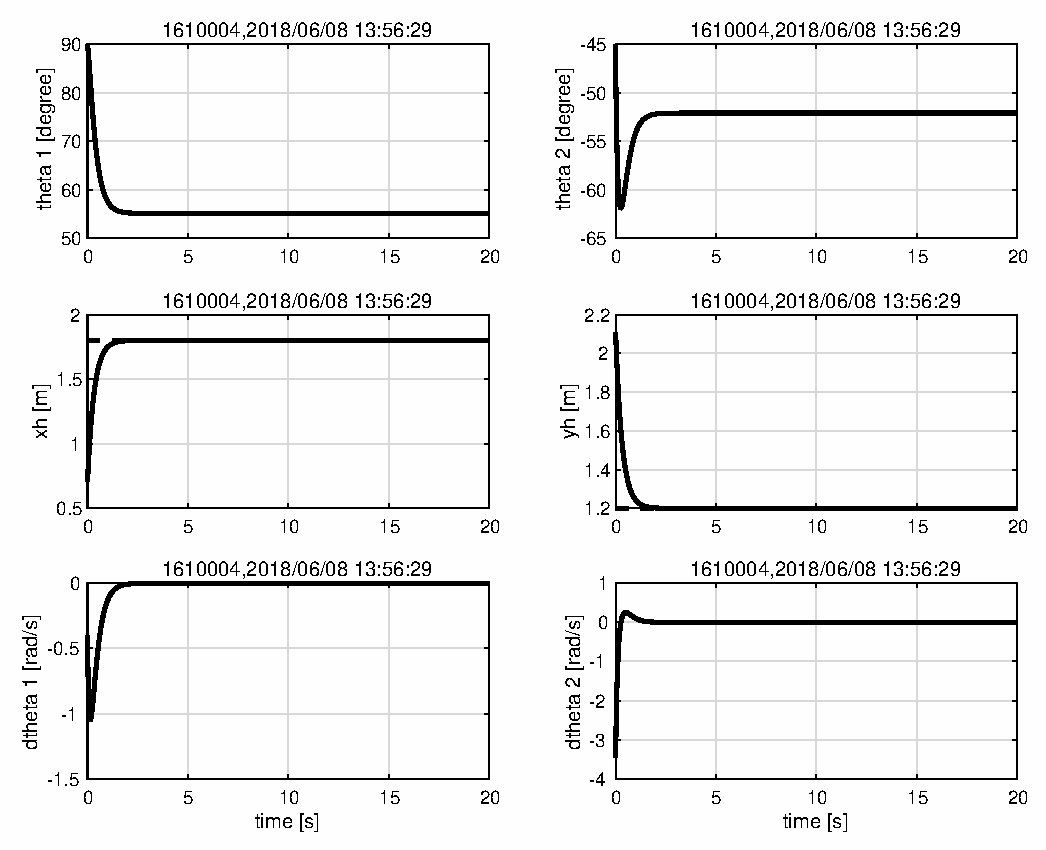
\includegraphics[width = 9cm]{画像/eps_手先_時不変_時間応答}
    \caption{シミュレーション:時不変}
    \label{手先1}
  \end{center}
\end{figure}

\begin{figure}[H]
  \begin{center}
    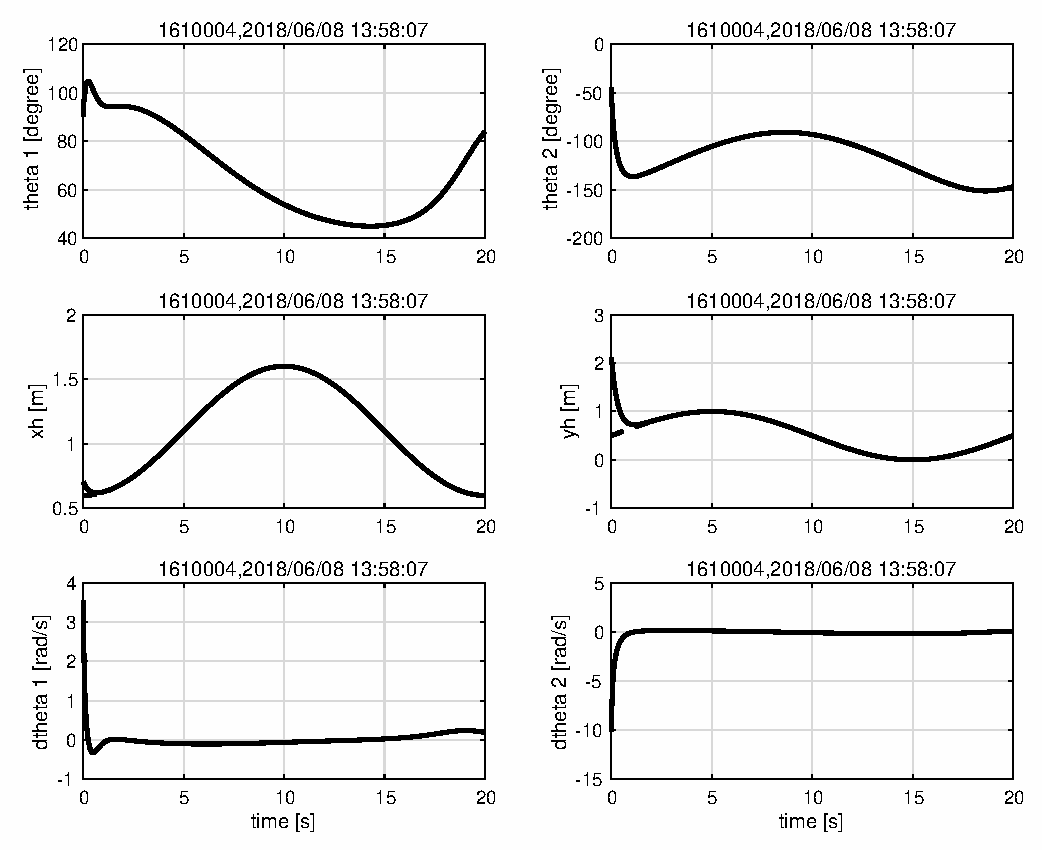
\includegraphics[width = 9cm]{画像/eps_手先_時変1_時間応答}
    \caption{シミュレーション:時変1}
    \label{手先2}
  \end{center}
\end{figure}

\begin{figure}[H]
  \begin{center}
    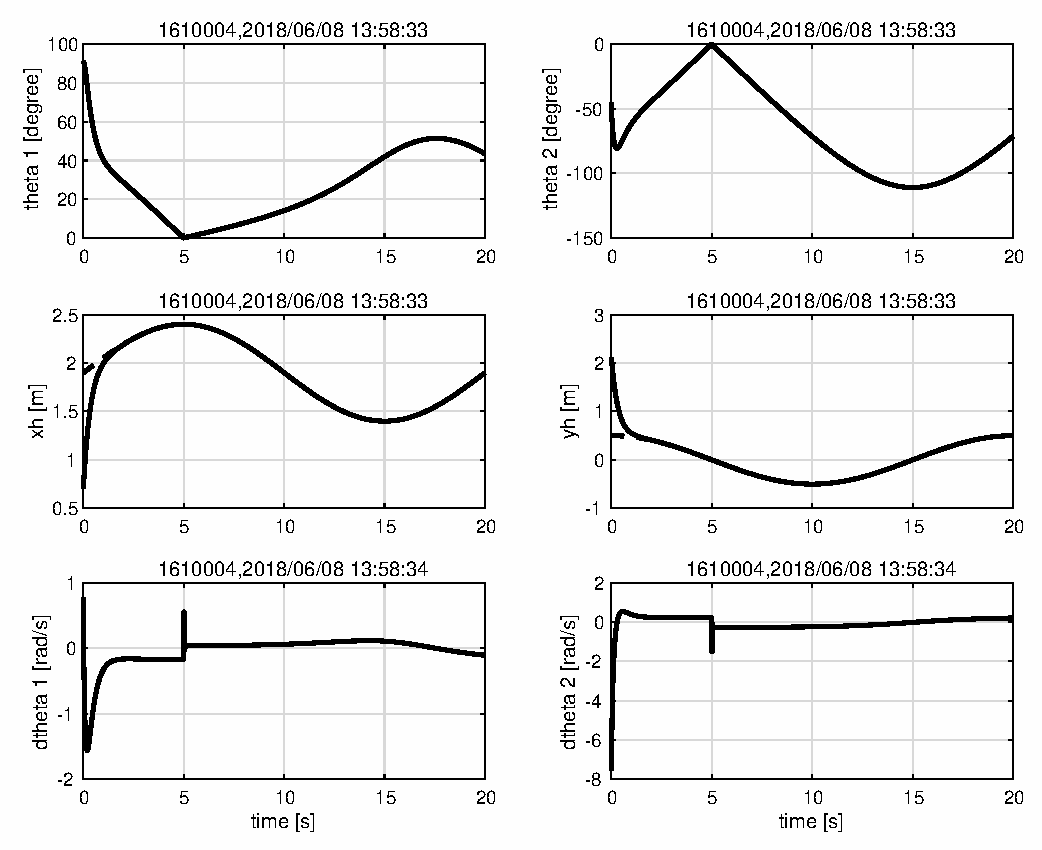
\includegraphics[width = 9cm]{画像/eps_手先_時変2_時間応答}
    \caption{シミュレーション:時変2}
    \label{手先3}
  \end{center}
\end{figure}

\begin{figure}[H]
  \begin{center}
    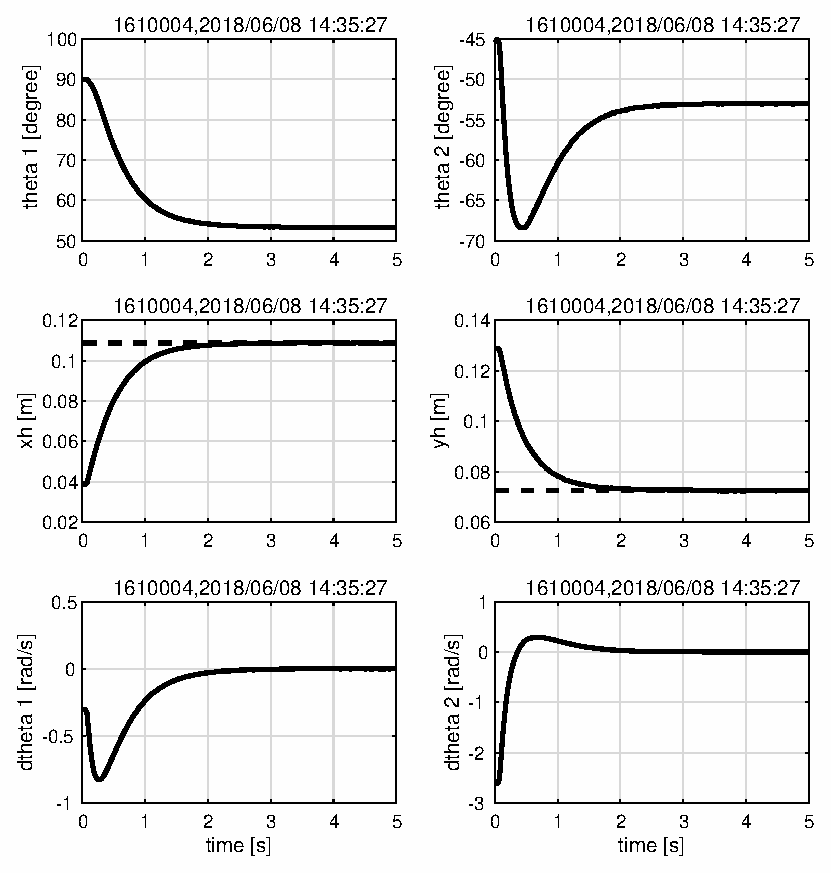
\includegraphics[width = 9cm]{画像/eps_実機実験_手先_時不変_時間応答}
    \caption{実機:時不変}
    \label{手先1/実機}
  \end{center}
\end{figure}

\begin{figure}[H]
  \begin{center}
    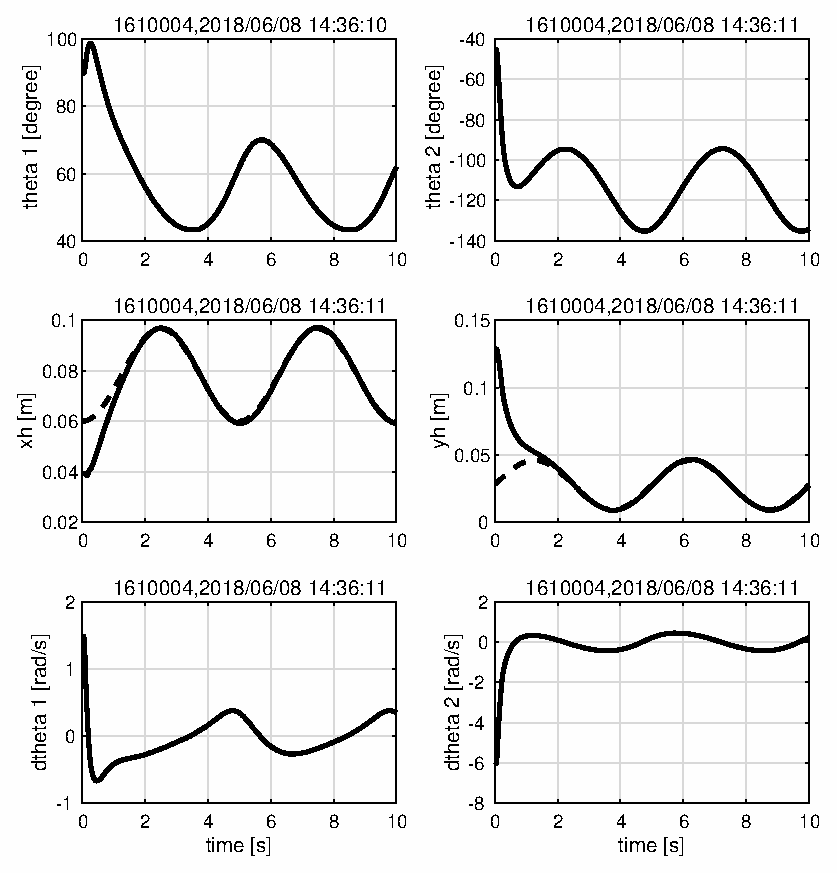
\includegraphics[width = 9cm]{画像/eps_実機実験_手先_時変1_時間応答}
    \caption{実機:時変1}
    \label{手先2/実機}
  \end{center}
\end{figure}

\begin{figure}[H]
  \begin{center}
    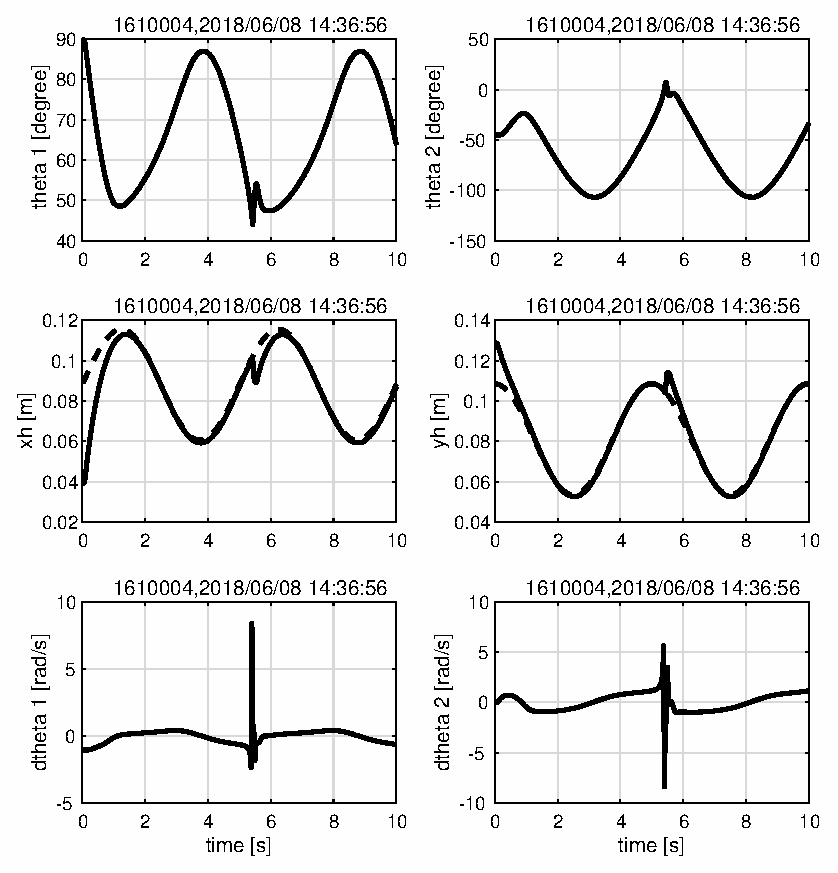
\includegraphics[width = 9cm]{画像/eps_実機実験_手先_時変2_時間応答}
    \caption{実機:時変2}
    \label{手先3/実機}
  \end{center}
\end{figure}

シミュレーションの目標値が時不変,時変1(\ref{手先1},\ref{手先2})の場合では滑らかに目標値に制御できているが,時変2(図\ref{手先3})の場合では急激なずれが生じている.
これは目標地点に向かう際(t=5), ロボットが特異点となる姿勢になってしまったために正常な制御ができなくなっていると考えられる.
実機でも同様に, 時変2(\ref{手先3/実機})のt=5において確かに特異点となったと思われる点が見られる.
\par
シミュレーションと実機の違いについて考察する.
時変2の場合,特異点に達した後, シミュレーションではすぐにリカバリーできているのに対し, 実機では特異点に達した後,
リカバリーするまでに少し時間がかかっている. これは, 実機とシミュレーションの間にモデル誤差が生じていたため, 正確に制御できるまで時間がかかってしまったことよると思われる.

\subsection{課題5}
冗長ロボットアームを対象に,条件無使用,衝突回避,関節角度減少化,衝突回避+関節角度減少化と変更して制御を実行し,結果を観察した.
その結果を以下に示す.

\begin{figure}[H]
  \begin{center}
    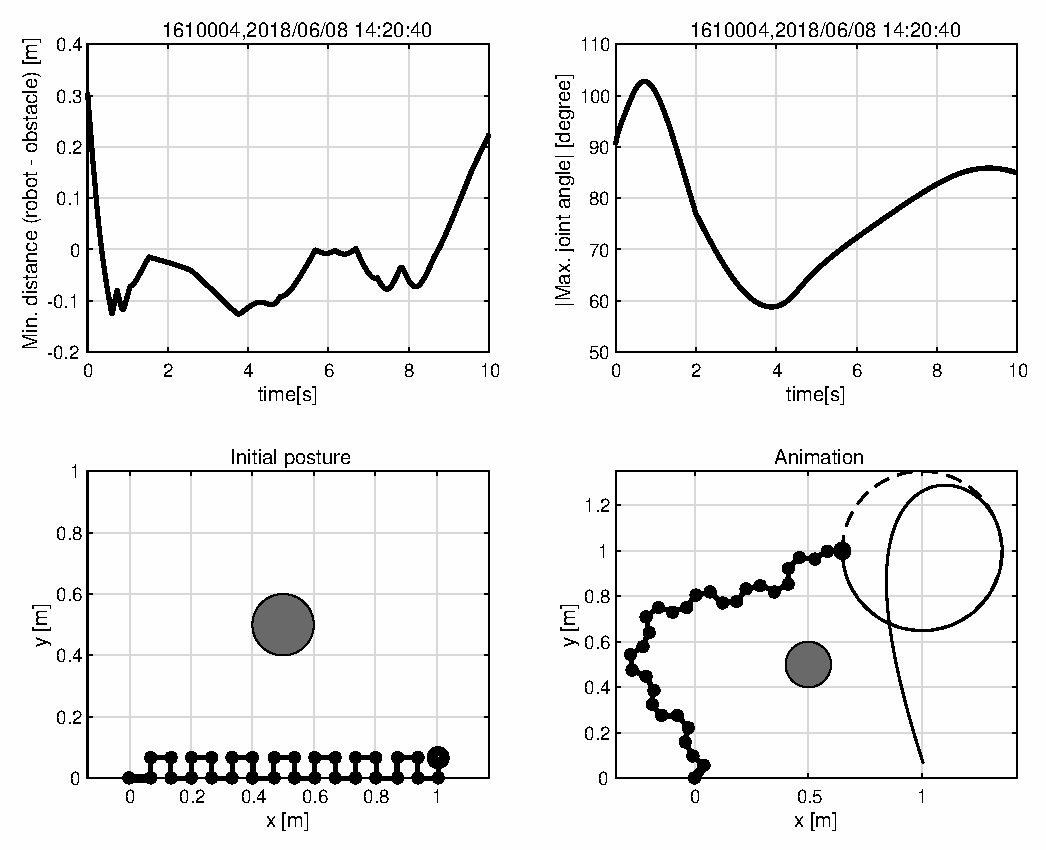
\includegraphics[width = 10cm]{画像/eps_冗長_未使用_結果}
    \caption{条件:未使用}
    \label{未使用}
  \end{center}
\end{figure}

\begin{figure}[H]
  \begin{center}
    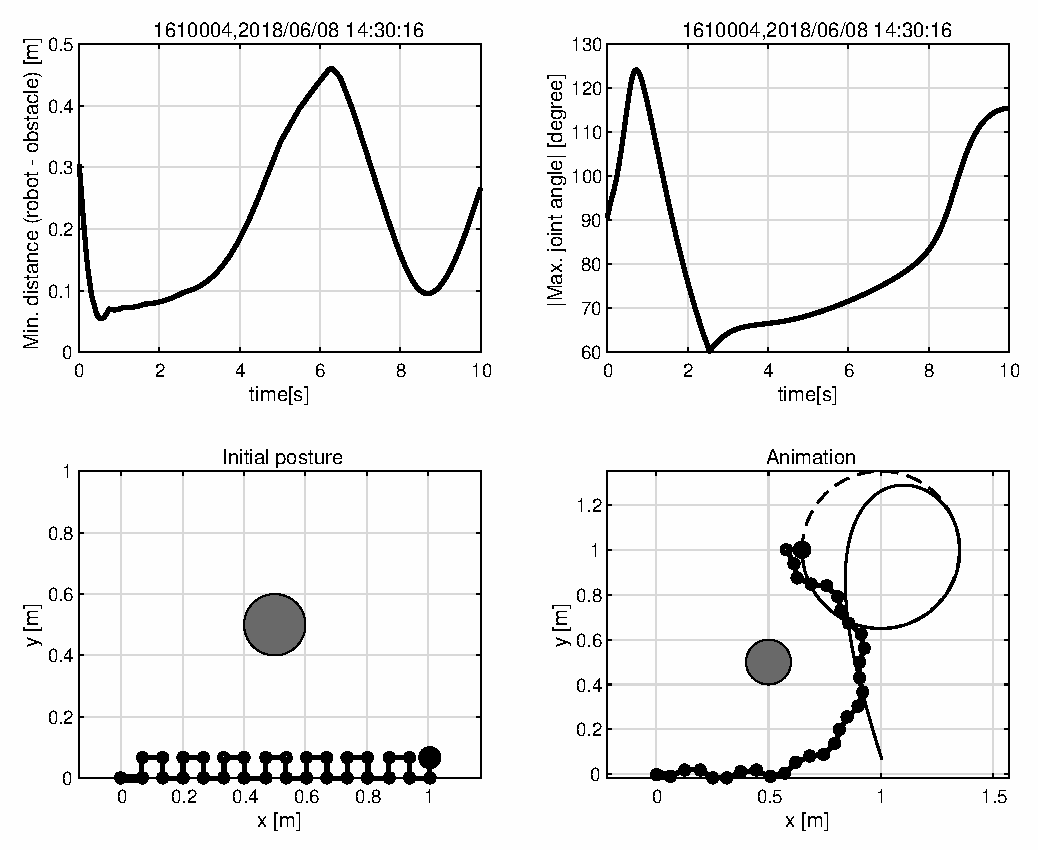
\includegraphics[width = 10cm]{画像/eps_冗長_衝突回避_結果}
    \caption{条件:衝突回避}
    \label{衝突回避}
  \end{center}
\end{figure}


\begin{figure}[H]
  \begin{center}
    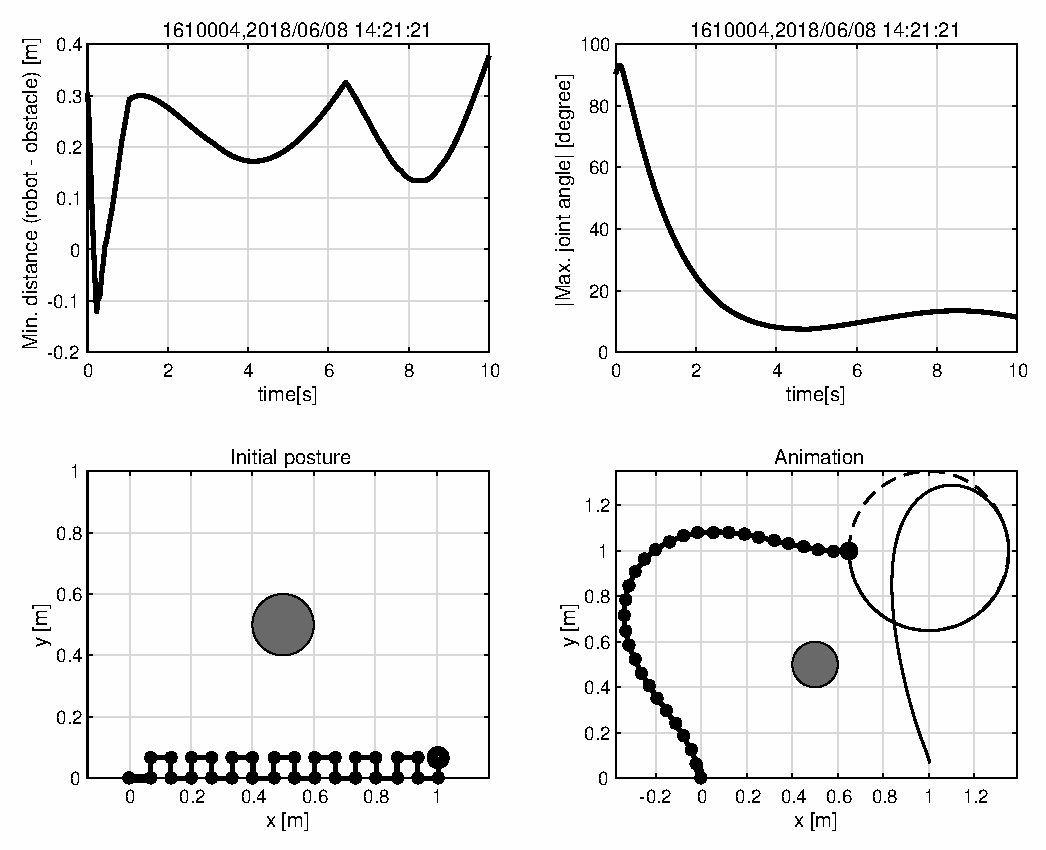
\includegraphics[width = 10cm]{画像/eps_冗長_関節角度減少化_結果}
    \caption{条件:関節角度減少化}
    \label{関節角度減少化}
  \end{center}
\end{figure}

\begin{figure}[H]
  \begin{center}
    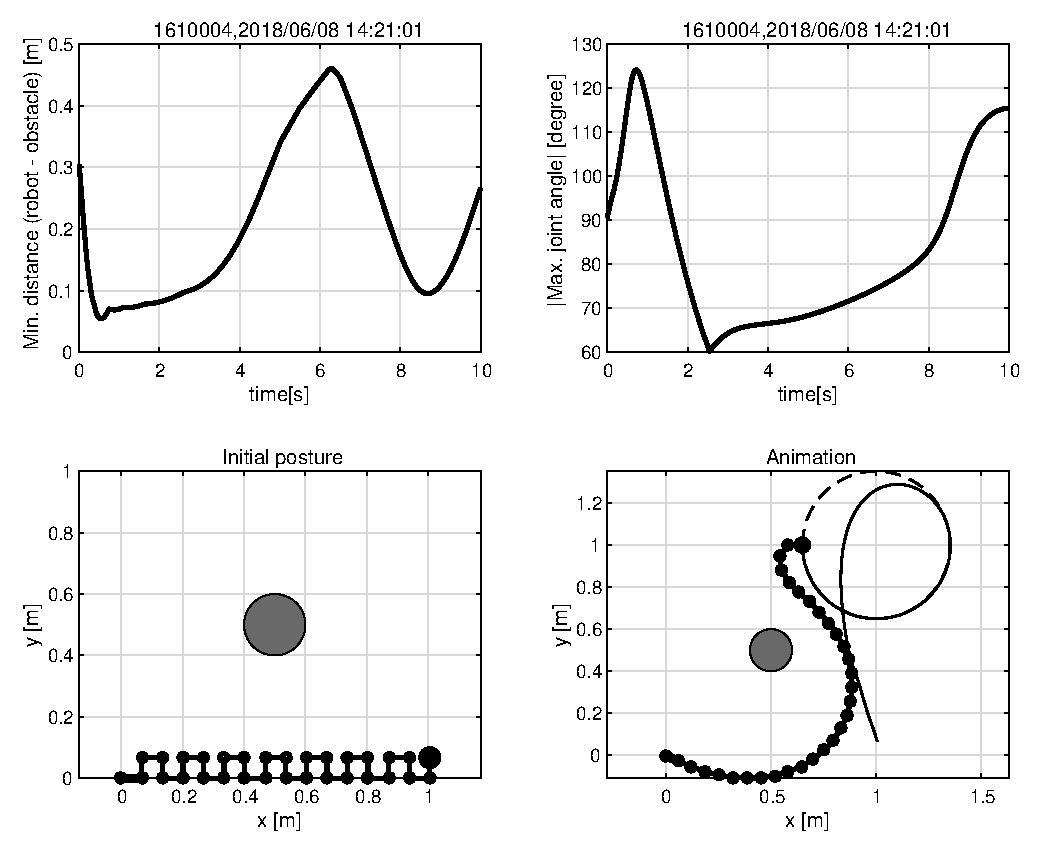
\includegraphics[width = 10cm]{画像/eps_冗長_衝突回避+関節角度減少化_結果}
    \caption{条件:衝突回避+関節角度減少化}
    \label{衝突回避+関節角度減少化}
  \end{center}
\end{figure}

それぞれの条件と制御結果について考察する.
まず未使用の場合(図\ref{未使用})では目標値通りに制御できているが, 障害物とロボットの距離の最小値を示したグラフを見ると
負の値,つまり衝突してしまっていることがわかる.これは制御パラメータの中に障害物との距離が考慮されていないためによるものである.
そこで,衝突回避の条件を付加した場合(\ref{衝突回避})について見る.未使用の場合とほぼ変わらない精度で制御できており, 障害物とロボットの距離の最小値も0を下回っていない.
しかしながら, 関節角度の最小値は,未使用の場合では滑らかなグラフ,つまり関節への負荷が小さいのに対し, 衝突回避の場合では2.5秒付近で大きな負荷がかかってしまっていることがわかる.
次に関節角度減少化の条件について考える.こちらも未使用の場合と精度はほぼ変わっていないが,さらに関節角度の変化が滑らかになっており,関節への負荷が少ない.
しかし,障害物と衝突してしまっている.最後に,衝突回避と関節角度最小化を組み合わせた制御について見ていく.この条件の時にはロボットと障害物の最小値のグラフは
衝突回避の場合と一致し, 関節角度の最大値のグラフは関節角度最小化の場合と一致している.
つまり, 制御パラメータに実現したい制御を満たすような条件を付加していくことで改善できることがわかる.

\section{レポート課題}
\subsection{課題A:ロボット制御における「特異点」「特異姿勢」の種類を数学的意味,物理的意味を交えて説明する.
また,「特異点」「特異姿勢」を回避するための方法を説明する.}
「特異点」「特異姿勢」はロボットがある特定の姿勢に達した際に, 制御するための解が計算不可能になり, 一時的に制御不能になる点のことである.
ここで, 特異点について数学的に説明していく.原点からロボットの手先位置へのベクトルを$\bm{P}$
とし,各関節角の変位のベクトルを$\bm{\theta}$とすると,出力点の速度に対する関節角の変位の速度はヤコビ行列を用いて次のように表される.
\begin{align}
  \bm{\dot{\theta}} = \bm{J}^{-1} \cdot \bm{\dot{P}}
\end{align}
この式が解を持つためには$\bm{J}^{-1}$に逆行列が存在している必要がある.逆に$\bm{J}^{-1}$の逆行列が存在しない場合,
すなわち以下の式が成り立つ時, 入力に対して出力不可能な姿勢となる.[1]
\begin{align}
  det\bm{J}^{-1} = 0
\end{align}
このことを次に示す2自由度マニピュレータリンク(図\ref{2自由度})を例にとって考えてみる.
\begin{figure}[H]
  \begin{center}
    \includegraphics[width = 10cm]{画像/2自由度.png}
    \caption{2自由度マニピュレータリンク}
    \label{2自由度}
  \end{center}
\end{figure}
このマニピュレータリンクのヤコビ行列は次のようになる.
\begin{align}
  \left[
	\begin{array}{cc}
		-l_1\sin{q_1}-l_2\sin(q_1+q_2) & -l_2\sin(q_1+q_2) \\
    l_1\cos{q_1}+l_2\cos(q_1+q_2) & l_2\cos(q_1+q_2)
	\end{array}
	\right]
\end{align}
このヤコビ行列の行列式を求めると以下のようになる.
\begin{align}
  det\bm{J}^{-1} = l_1l_2\sin{q_2}
\end{align}
すなわち, $q_2 = 0^{\circ}, 180^{\circ}$の時, このマニピュレータリンクは特異点となる.
$q_2=0^{\circ}$の時,アームが伸びきった状態になってしまう(図\ref{0degree}).
\begin{figure}[H]
  \begin{center}
    \includegraphics[width = 10cm]{画像/0degree.png}
    \caption{0degree}
    \label{0degree}
  \end{center}
\end{figure}


$q_2=180^{\circ}$の時,アームが伸びきった状態になってしまう(図\ref{180degree}).
\begin{figure}[H]
  \begin{center}
    \includegraphics[width = 10cm]{画像/180degree.png}
    \caption{180degree}
    \label{180degree}
  \end{center}
\end{figure}

以上二つの状態を見ると,2自由度であるのに関わらず, 1自由度の運動しかできない状態になっていることがわかる.[2]

\subsection{課題B:「今年度」または「昨年度」に行われたロボットの研究論文の調査}

\subsubsection{各種情報}
論文タイトル: Smooth joint motion planning for high precision reconfigurable robot manipulators,研究機関:University of Applied Sciences and Arts of Southern Switzerland (SUPSI),\\研究者:S.Baraldo, A.Valente, 雑誌名:IEEE
\subsubsection{研究目的}
現代で生じている急速な技術革新に工業用ロボットを対応させるためには,再構成可能な設計をしなくてはならない.
しかしながら,高精度かつ信頼性の高い,再構成可能な設計は依然として主要課題のままである.
そのため,この研究では精密性と再構成可能という性質を兼ね備えた,あらゆる作業に対応可能なマニピュレータ"ReRob I"の設計,制御の実現を目的とする.
\subsubsection{ロボットの構造}
作業を実行可能な性能とサイズからリンクとアクチュエータの両方を選定することで再構成可能にしている.
ReRob Iは2種類のジョイントから構成されており,高トルクの3つのジョイントと低トルクの3つのジョイントからなっている.

\begin{figure}[H]
  \begin{center}
    \includegraphics[width = 10cm]{画像/ReRob.png}
    \caption{ReRobの概形}
    \label{ReRob}
  \end{center}
\end{figure}

\subsubsection{制御方法}
滑らかな軌道とアームに生じる不要な振動や負荷を軽減する動きを実現するために,ジャーク、加速度、速度を固定値のままにしながら、すべてのジョイントのモーションプロファイルを同期させて同時に移動を完了させる.
これはすべての6つの関節のモーションプロファイルを一度に考慮に入れ、非線形補償付き最適化を設定することに相当しており,
特定の作業要件と並行して、キネマティックチェーンの相対ジョイント位置に関するモーション機能を活用する.

\subsubsection{得られた結果}
この制御方法を用いることで, モーションプロファイルを滑らかに維持しながら,現在最善とされている方法よりも39\%以上短い時間で作業を実行することができた.

\subsubsection{感想と意見}
再構成可能にしたというロボットの構造がなぜ再構成可能なのかが理解しきれなかった.また, 制御方法について述べられている部分もどのような制御構造になっているのか, なにが従来と革新的に違うのかが理解できなかった.


\section{参考文献}
[1]金沢大学 理工学域 機械工学類 機械機能設計研究室HPより,URL:http://da.ms.t.kanazawa-u.ac.jp/lab/tachiya/text/robot/2.pdf
[2]明 愛国:Webclass:ロボットの機構と力学

\section{実験に対する意見・感想}
全体を通して, ロボットの特徴や問題点について体形だった実験であったので理解しやすく, 今までの学習した事柄について総ざらいできたため, 大変勉強になった.
課題1, 2における時変と不時変による制御結果の違いの考察がうまくできず心残りである.
課題4, 5では講義で学んだ特異点について実際に実機でどのように動作するのか確認できたことが非常に興味深かった.

\end{document}
